\documentclass[12pt]{beamer}
\newenvironment{ConCodigo}[1]
  {\begin{frame}[fragile,environment=ConCodigo]{#1}}
  {\end{frame}}
\graphicspath{{Imagenes/}{../Imagenes/}}
\usepackage[utf8]{inputenc}
\usepackage[spanish]{babel}
\usepackage{hyperref}
\usepackage{etex}
\reserveinserts{28}
\usepackage{amsmath}
\usepackage{amsthm}
\usepackage{mathtools}
\usepackage{multicol}
\usepackage{multirow}
\usepackage{tabulary}
\usepackage{booktabs}
\usepackage{nccmath}
\usepackage{biblatex}
\usepackage{epstopdf}
\usepackage{graphicx}
%\usepackage{enumitem,xcolor}
\usepackage{siunitx}
\sisetup{scientific-notation=true}
%\usepackage{fontspec}
\usepackage{lmodern}
\usepackage{float}
\usepackage[format=hang, font=footnotesize, labelformat=parens]{caption}
\usepackage[autostyle,spanish=mexican]{csquotes}
\usepackage{standalone}
\usepackage{blkarray}
\usepackage{algorithm}
\usepackage{algorithmic}
\usepackage{tikz}
\usepackage[siunitx]{circuitikz}
\usetikzlibrary{arrows,patterns,shapes}
\usetikzlibrary{decorations.markings}
\usetikzlibrary{arrows}
\usepackage{color}
\usepackage{xcolor}
%\usepackage{beton}
%\usepackage{euler}
%\usepackage[T1]{fontenc}
\usepackage[sfdefault]{roboto}  %% Option 'sfdefault' only if the base font of the document is to be sans serif
\usepackage[T1]{fontenc}
\renewcommand*\familydefault{\sfdefault}
\DeclareGraphicsExtensions{.pdf,.png,.jpg}
\usepackage{hyperref}
\renewcommand {\arraystretch}{1.5}
\newcommand{\python}{\texttt{python}}
\usefonttheme[onlymath]{serif}
\setbeamertemplate{navigation symbols}{}
\usetikzlibrary{patterns}
\usetikzlibrary{decorations.markings}
\tikzstyle{every picture}+=[remember picture,baseline]
%\tikzstyle{every node}+=[inner sep=0pt,anchor=base,
%minimum width=2.2cm,align=center,text depth=.15ex,outer sep=1.5pt]
%\tikzstyle{every path}+=[thick, rounded corners]
\setbeamertemplate{caption}[numbered]
\newcommand{\ptm}{\fontfamily{ptm}\selectfont}
%Se usa la plantilla Warsaw modificada con spruce
\mode<presentation>
{
  \usetheme{Warsaw}
  \setbeamertemplate{headline}{}
  \useoutertheme{default}
  \usecolortheme{seahorse}
  \setbeamercovered{invisible}
}
% \AtBeginSection[]
% {
% \begin{frame}<beamer>{Contenido}
% \normalfont\mdseries
% \tableofcontents[currentsection]
% \end{frame}
%}

\usepackage{listings}
\lstset{ %
language=Python,                % choose the language of the code
basicstyle=\small,       % the size of the fonts that are used for the code
numbers=left,                   % where to put the line-numbers
numberstyle=\footnotesize,      % the size of the fonts that are used for the line-numbers
stepnumber=1,                   % the step between two line-numbers. If it is 1 each line will be numbered
numbersep=5pt,                  % how far the line-numbers are from the code
backgroundcolor=\color{white},  % choose the background color. You must add \usepackage{color}
showspaces=false,               % show spaces adding particular underscores
showstringspaces=false,         % underline spaces within strings
showtabs=false,                 % show tabs within strings adding particular underscores
frame=single,   		% adds a frame around the code
tabsize=4,  		% sets default tabsize to 2 spaces
captionpos=b,   		% sets the caption-position to bottom
breaklines=true,    	% sets automatic line breaking
breakatwhitespace=false,    % sets if automatic breaks should only happen at whitespace
escapeinside={\#}{)}          % if you want to add a comment within your code
}

\begin{document}
\title{Tema 0 - Programación Básica con \python}
\subtitle{Curso de Física Computacional}
\author[]{M. en C. Gustavo Contreras Mayén}
\institute{Facultad de Ciencias - UNAM}
\titlegraphic{
\includegraphics[width=2cm]{escudo-facultad-ciencias.jpg}\hspace*{4.75cm}~%
   
\includegraphics[width=2cm]{escudo-unam.jpg}
}
\date{\today}
\maketitle
\fontsize{14}{14}\selectfont
\spanishdecimal{.}
\section*{Contenido}
\frame{\tableofcontents[currentsection, hideallsubsections]}
\section{Introducción}
\begin{frame}
Para el curso de Física Computacional será necesario que usemos un lenguaje de programación para apoyarnos en la solución de los problemas.
\\
\bigskip
El lenguaje de nuestra elección es un medio para alcanzar nuestro objetivo del curso, más no el fin, por lo que revisaremos lo más básico de \python, dando la oportunidad de que por tu cuenta, logres un mayor conocimiento y práctica con \python.
\\
\bigskip
Si ya cuentas con el conocimiento y práctica de algún otro lenguaje, podrás trabajar con él, para ello, deberás de enviar detallado tu archivo con el código, así como con el ejecutable.
\end{frame}
\begin{frame}
\begin{figure}
	\centering
	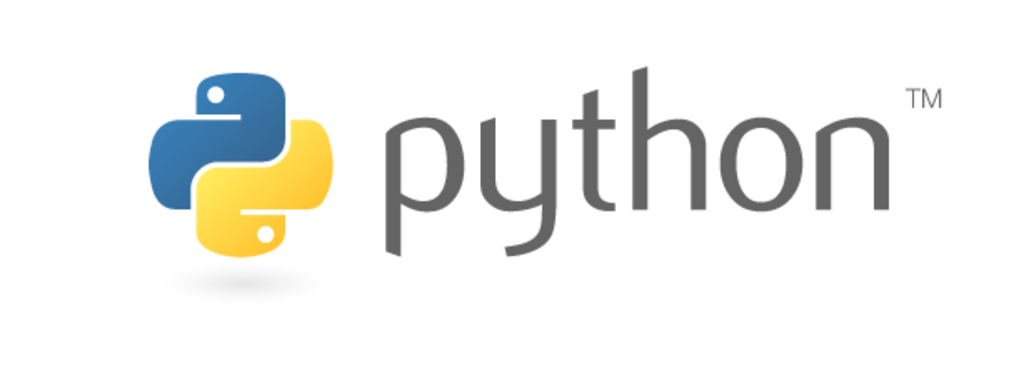
\includegraphics[scale=0.5]{python-logo-master-v3-TM2.eps} 
\end{figure}
\begin{uncoverenv}
\begin{itemize}[<+->]
\item Lenguaje de programación de alto nivel, interpretado.
\item Desarrollado por Guido van Rossum a principios de
los años 90.
\item Es multiplataforma (UNIX, Solaris, Linux, DOS, Windows, OS/2, Mac OS, etc.)
\item Software libre: Python Software Foundation License (PSFL)
\end{itemize}
\end{uncoverenv}
\end{frame}
\begin{frame}
\begin{uncoverenv}
\begin{itemize}[<+->]
\item Es usado en todo tipo de aplicaciones: científicas, administración de sistemas, procesamiento de texto, páginas web, bases de datos, visualización 3D y videojuegos, inteligencia artificial, etc.
\item Presenta una sintaxis compacta, sencilla e intuitiva, una curva de aprendizaje mínima (comparada por ejemplo contra Fortran o Java), junto a una potente librería de funciones y clases.
\item Lo anterior permite programar una aplicación completa en cuestión de horas o incluso minutos.
\end{itemize}
\end{uncoverenv}
\end{frame}
\begin{frame}
\frametitle{¿Por qué usar \python\ 3?}
\begin{itemize}[<+->]
\item Tiene un diseño simple e internamente consistente.
\item El código es muy claro y legible.
\item Es un lenguaje de alto nivel: operaciones complejas en muy pocas líneas.
\item Cuenta con módulos que facilitan un amplio espectro de tareas.
\item Versatilidad: distintos paradigmas de programación: estructurada, orientada a objetos, funcional.
\end{itemize}
\end{frame}
\begin{frame}
\frametitle{Simplicidad como filosofía base}
\begin{enumerate}
\item Bello es mejor que feo.
\item Explícito es mejor que implícito.
\item Simple es mejor que complejo.
\item Complejo es mejor que complicado.
\item Plano es mejor que anidado.
\item Disperso es mejor que denso.
\item La legibilidad cuenta.
\item \ldots
\end{enumerate}
El código que sigue los principios de \python\ de legibilidad y transparencia se dice que es ''pythonico". Contrariamente, el código opaco u ofuscado es bautizado como ''no pythonico" %(''un\pythonic" en inglés).
\end{frame}
\begin{frame}[fragile]
\frametitle{\python y otros lenguajes de programación}
Para calcular el factorial de un número en \texttt{C}:
\begin{verbatim}
int factorial(int x)
{
    if (x == 0)
        return 1;
    else
        return x * factorial(x - 1);
}
\end{verbatim}
En \python:
\begin{verbatim}
def factorial(x):
    if x == 0:
        return 1
    else:
        return x * factorial(x - 1)
\end{verbatim}

\end{frame}
%\begin{frame}
%\frametitle{La sintaxis de \python}
%La sintaxis de \python\ 2.7.x se compone de 35 palabras
%\begin{multicols}{3}
%\texttt{
%and \\
%as \\
%assert \\
%break \\
%class \\
%continue \\
%def \\
%del \\
%elif \\
%else \\
%except \\
%exec \\
%False \\
%finally \\
%for \\
%from \\
%global \\
%if \\
%import \\
%in \\
%is \\
%lambda \\
%None \\
%nonlocal \\
%not \\
%or \\
%pass \\
%print \\
%raise \\
%return \\
%True \\
%try \\
%while \\
%with \\
%yield }
%\end{multicols}
%\end{frame}
\begin{frame}
\frametitle{Filosofía de ''pilas incluidas"}
La librería estándar de \python\ incluye módulos para:
\begin{itemize}
\item Funciones matemáticas reales y complejas, números aleatorios, criptografía.
\item Manejo de conexiones de red (TCP/IP, Web, FTP, correo, etc.)
\item Compresión y descompresión de archivos (zlib, gzip, bzip2, tar)
\item Manipulación de texto y expresiones regulares.
\item Acceso a bases de datos.
\item Acceso al sistema operativo, creación de subprocesos, manejo de archivos y directorio.
\end{itemize}
\end{frame}
\section{Características de \python}
\begin{frame}
\frametitle{Características de \python}
Algunas de las principales características de \python\ que lo convierten en un lenguaje versátil, son:
\begin{itemize}
\item Tipado dinámico.
\item Fuertemente tipado.
\item Orientado a objetos.
\end{itemize}
\end{frame}
\begin{frame}
\frametitle{Tipado dinámico}
Cada dato es de un tipo determinado y sólo se puede operar con él de formas bien definidas.
\\
\bigskip
La ventaja es que \textcolor{red}{NO hay que declarar variables antes de su uso}.
\end{frame}
\begin{frame}
\frametitle{Fuertemente tipado}
Se dice que es un lenguaje cuyos tipos son estrictos. Java y \python\ son fuertemente tipados.
\\
\bigskip
Si se tiene un tipo de dato entero, no se puede tratar como una cadena de texto sin convertirlo explícitamente.
\end{frame}
\begin{frame}
\frametitle{Programación orientada a objetos}
La programación orientada a objetos es un paradigma de programación que busca representar entidades u objetos agrupando datos y métodos que puedan describir sus características y comportamientos.
\end{frame}
\begin{frame}[fragile]
\frametitle{Complementos para \python}
\begin{itemize}[<+->]
\item \visible<2->{NumPy: paquete fundamental para computación científica.}
\item \visible<3->{SciPy: librería para computación científica (extiende a NumPy)}
\item \visible<4->{matplotlib: librería para gráficos 2D (soporta gráficos 3D también)}
\item \visible<5->{Mayavi: librería para gráficos y visualización de datos 3D.}
\item \visible<6->{ipython: consola interactiva para \python.}
\end{itemize}
\end{frame}
\begin{frame}
\begin{figure}
	\centering
	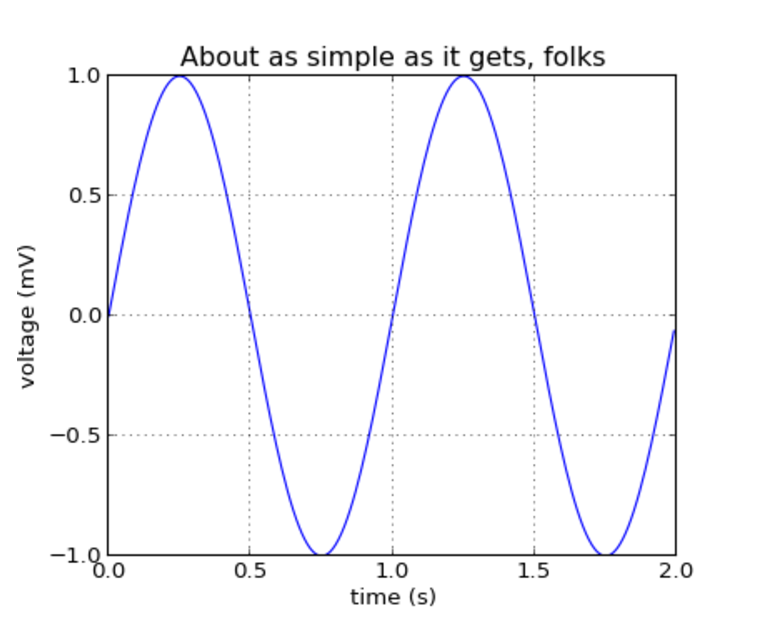
\includegraphics[scale=0.5]{simple_plot1.eps}<1> 
	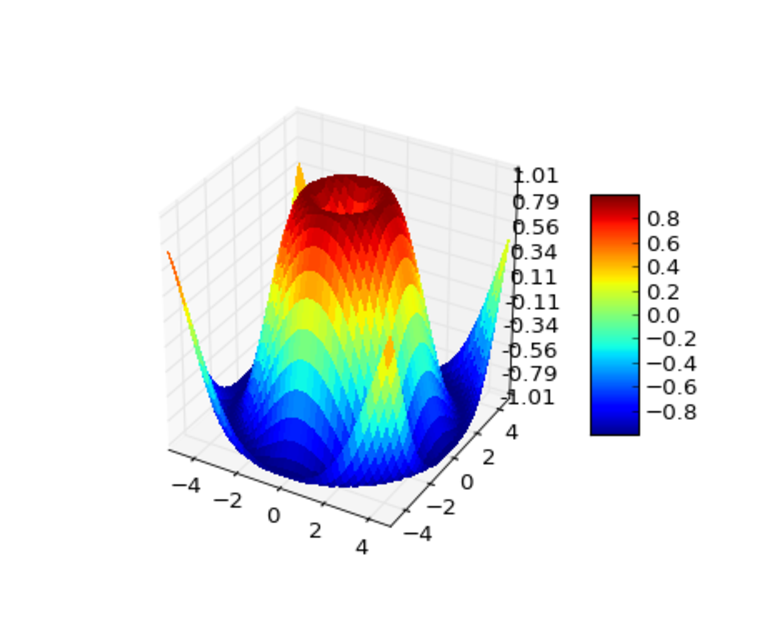
\includegraphics[scale=0.5]{surface3d_demo4.eps}<2>
	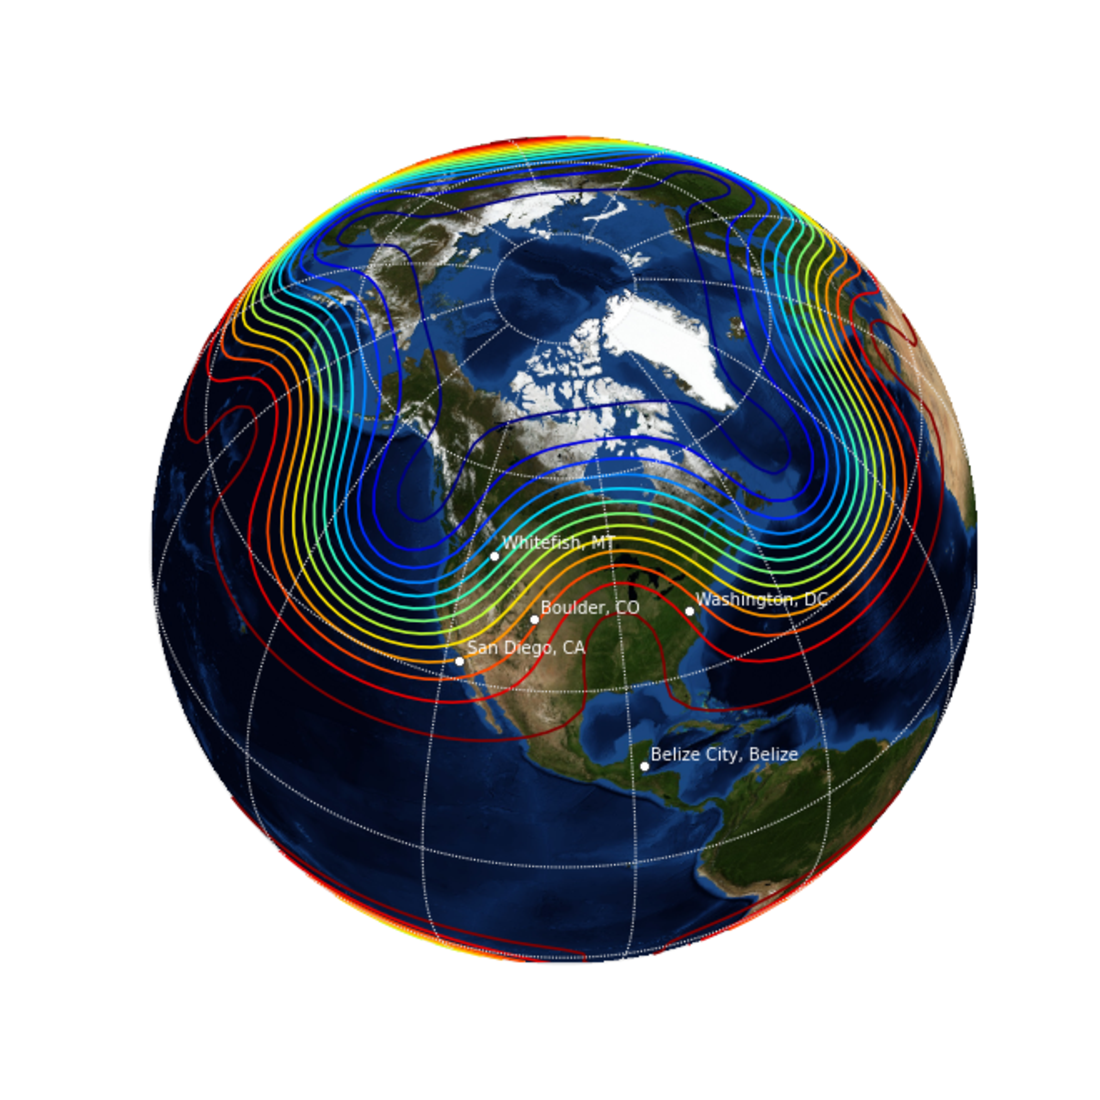
\includegraphics[scale=0.5]{plotmap.eps}<3>
\end{figure}
\end{frame}
\section{Trabajando con \python}
\begin{frame}
\frametitle{Trabajando con \python}
Hay dos modos de trabajo en \python, cada uno de ellos depende de nuestra habilidad:
\begin{itemize}[<+->]
\item \textbf{Modo rudo}: trabajo directo en la consola (uso del intérprete interactivo), sirve para probar pequeñas instrucciones, depurar programas, o buscar ayuda de funciones y métodos.
\item \textbf{Modo amigable}: a través de una interface IDLE (Entorno de Desarrollo Integrado), usando el código como un programa o script independiente, en el caso de un programa en su forma final o que ya tenga definidas funciones y clases propias.
\end{itemize}
\end{frame}
%\begin{frame}
%\frametitle{Modo Rudo}
%Se invoca la consola desde la terminal o consola de comandos, tecleando \texttt{python}
%\begin{figure}
%	\centering
%	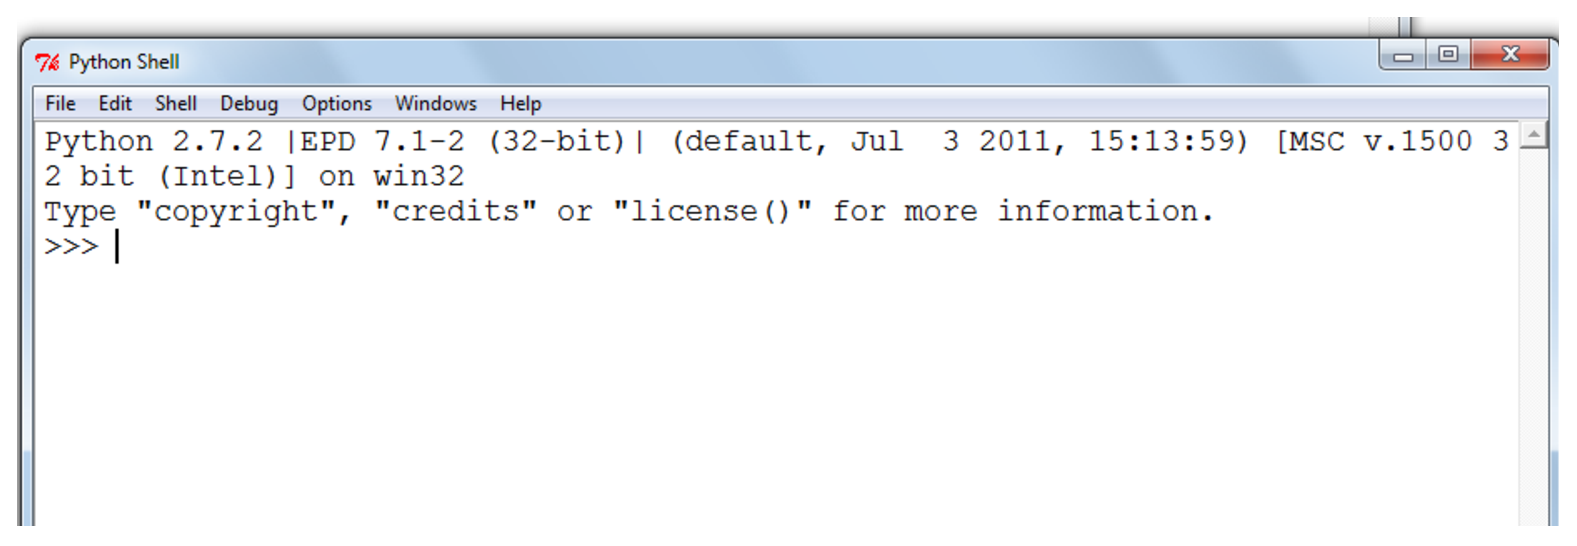
\includegraphics[scale=0.45]{pantalla01.eps} 
%\end{figure}
%\end{frame}
\begin{frame}[fragile]
\frametitle{¿Qué podemos hacer en el modo interactivo?}
\begin{itemize}
\item El prompt \verb|>>>| indica que \python\ está listo para recibir instrucciones.
\item Si tecleamos una expresión, ésta se evalúa y se muestra directamente el resultado.
\item La ayuda para una función se obtiene con \texttt{help} y el nombre de la función (entre paréntesis)
\\
\verb|>>> help(float)|
\item La ayuda para una palabra clave se obtiene con \texttt{help} y la palabra (entre comillas simples y paréntesis) 
\\
\verb|>>> help('while')|
\item Llamar a \texttt{help()} (sin argumentos) accede a la ayuda interactiva.
\end{itemize}
\end{frame}
\begin{frame}[fragile]
\frametitle{Programa o \textit{script} independiente}
\begin{lstlisting}
# Este es un programa o script en Python
# En una linea , todo lo que sigue a
# continuacion de un caracter # es comentario

print "Hola , Mundo !"

x = 42

print x + 8 # imprime 50

print 'Programar es divertido de nuevo'.split()

print ([x**2 for x in range (15)])
print ([x**2 for x in range (15) if x % 2 == 0])
\end{lstlisting}
\end{frame}
%\subsection{Operadores artiméticos}
%\begin{frame}
%\frametitle{\python\ como calculadora}
%Una vez abierta la sesión en \python, podemos aprovechar al máximo este lenguaje: contamos con una calculadora a la mano, sólo hay que ir escribiendo las operaciones en la línea de comandos.
%\end{frame}
%\begin{frame}[fragile]
%\frametitle{Operadores artiméticos}
%\begin{minipage}{5.5cm}
%\begin{exampleblock}{}<1->
%	\verb|>>> 3+4| \\
%	\visible<2->{\textcolor{blue}{\texttt{7}}}
%\end{exampleblock}
%\begin{exampleblock}{}<3->
%	\verb|>>> 3/4| \\
%	\visible<4->{\textcolor{blue}{\texttt{0}}}
%\end{exampleblock}
%\begin{exampleblock}{}<5->
%	\verb|>>> 3.0/4.0| \\
%	\visible<6->{\textcolor{blue}{\texttt{0.75}}}
%\end{exampleblock}
%\begin{exampleblock}{}<7->
%	\verb|>>> 5.0 / 10 * 2 + 5| \\
%	\visible<8->{\textcolor{blue}{\texttt{6}}}
%\end{exampleblock}
%\end{minipage}
%\end{frame}
%\begin{frame}[fragile]
%\frametitle{Operadores artiméticos}
%\begin{minipage}{5.5cm}
%\begin{exampleblock}{}<1->
%	\verb|>>> 5.0 / (10 * 2 + 5)| \\
%	\visible<2->{\textcolor{blue}{\texttt{0.2}}}
%\end{exampleblock}
%\begin{exampleblock}{}<3->
%	\verb|>>> 2**3**2| \\
%	\visible<4->{\textcolor{blue}{\texttt{512}}}
%\end{exampleblock}
%\begin{exampleblock}{}<5->
%	\verb|>>> (2**3)**2| \\
%	\visible<6->{\textcolor{blue}{\texttt{64}}}
%\end{exampleblock}
%\begin{exampleblock}{}<7->
%	\verb|>>> 17%3%2| \\
%	\visible<8->{\textcolor{blue}{\texttt{0}}}
%\end{exampleblock}
%\end{minipage}
%\end{frame}
%\begin{frame}
%\frametitle{Tabla de operadores}
%\begin{center}
%\begin{tabular}{| c | c | c | c |}
%\hline
%Operador & Operación & Ejemplo & Resultado \\
%\hline
%\hline
%$**$ & Potencia & $2**3$ & $8$ \\
%$*$ & Multiplicación & $7*3$ & 21 \\
%$/$ & División & $10.5/2$ & 5.25 \\
%$//$ & División entera & $10.5//2$ & 5.0 \\
%$+$ & Suma & $3+4$ & $7$ \\
%$-$ & Resta & $6-8$ & $-2$ \\
%$\%$ & Módulo & $15\%6$ & $3$ \\
%\hline
%\end{tabular}
%\end{center}
%\end{frame}
%\begin{frame}[fragile]
%\frametitle{Precedencia de operadores 1}
%\begin{enumerate}[<+->]
%\item Las expresiones contenidas dentro de pares de paréntesis son evaluadas primero. En el caso de expresiones con paréntesis anidados, los operadores en el par de paréntesis más interno son aplicados primero.
%\item Las operaciones de exponentes son aplicadas después. Si una expresión contiene muchas operaciones de exponentes, los operadores son aplicados de derecha a izquierda.
%\end{enumerate}
%\end{frame}
%\begin{frame}[fragile]
%\frametitle{Precedencia de operadores 2}
%\begin{enumerate}[<+->]
%\setcounter{enumi}{2}
%\item La multiplicación, división y módulo son las siguientes en ser aplicadas. Si una expresión contiene muchas multiplicaciones, divisiones u operaciones de módulo, los operadores se aplican de izquierda a derecha.
%\item Suma y resta son las operaciones que se aplican por último. Si una expresión contiene muchas operaciones de suma y resta, los operadores son aplicados de izquierda a derecha. La suma y resta tienen el mismo nivel de precedencia.
%\end{enumerate}
%\end{frame}
%\subsection{Operadores relacionales}
%\begin{frame}[fragile]
%\frametitle{Operadores relacionales (de comparación)}
%Tipos de datos lógicos: \texttt{False (0)} y \texttt{True (1)}
%\begin{minipage}{5.5cm}
%\begin{exampleblock}{}<1->
%	\verb|1+2>7-3| \\
%	\pause
%	\textcolor{blue}{\texttt{False}}
%\end{exampleblock}
%\begin{exampleblock}{}<2->
%	\verb|1<2<3| \\
%	\pause
%	\textcolor{blue}{\texttt{True}}
%\end{exampleblock}
%\begin{exampleblock}{}<3->
%	\verb|1>2==2<3| \\
%	\pause
%	\textcolor{blue}{\texttt{False}}
%\end{exampleblock}
%\begin{exampleblock}{}<4->
%	\verb|1>(2==2)<3| \\
%	\pause
%	\textcolor{blue}{\texttt{False}}
%\end{exampleblock}
%\end{minipage}
%\end{frame}
%\begin{frame}[fragile]
%\frametitle{Operadores relacionales (de comparación)}
%\begin{minipage}{5.5cm}
%\begin{exampleblock}{}<5->
%	\verb|3>4<5| \\
%	\pause
%	\textcolor{blue}{\texttt{False}}
%\end{exampleblock}
%\begin{exampleblock}{}<6->
%	\verb|1.0/3<0.33333| \\
%	\pause
%	\textcolor{blue}{\texttt{False}}
%\end{exampleblock}
%\begin{exampleblock}{}<7->
%	\verb|5.0/3>=11/7.0| \\
%	\pause
%	\textcolor{blue}{\texttt{True}}
%\end{exampleblock}
%\begin{exampleblock}{}<8->
%	\verb|2**(2./3)<3**(3./4)| \\
%	\pause
%	\textcolor{blue}{\texttt{True}}
%\end{exampleblock}
%\end{minipage}
%\end{frame}
%\begin{frame}
%\frametitle{Tabla de operadores relacionales}
%\begin{center}
%\begin{tabular}{| c | c | c | c |}
%\hline
%Operador & Operación & Ejemplo & Resultado \\
%\hline
%\hline
%$==$ & Igual a & $4==5$ & \texttt{False}  \\
%$!=$ & Diferente de & $2!=3$ & \texttt{True} \\
%$<$ & Menor que & $10<4$ & \texttt{False} \\
%$>$ & Mayor que & $5>-4$ & \texttt{True} \\
%$<=$ & Menor o igual que & $7<=7$ & \texttt{True} \\
%$>=$ & Mayor o igual que & $3.5 >= 10$ & \texttt{False} \\
%\hline
%\end{tabular}
%\end{center}
%\end{frame}
%\begin{frame}
%\frametitle{Operadores lógicos (booleanos)}
%\begin{center}
%\begin{tabular}{| c | c | c | c |}
%\hline
%Operador & Operación & Ejemplo & Resultado \\
%\hline
%\hline
%\texttt{and} & conjunción & \texttt{False and True} & \texttt{False} \\
%\texttt{or} & disyunción & \texttt{False or True} & \texttt{True} \\
%\texttt{not} & negación & \texttt{not True} & \texttt{False} \\
%\hline
%\end{tabular}
%\end{center}
%\end{frame}
%\begin{frame}
%\frametitle{Tabla de verdad}
%\texttt{
%\begin{center}
%\begin{tabular}{| c | c | c | c | c |}
%\hline
%A & B & A and B & A or B & not A \\
%\hline
%\hline
%True & True & True & True & False \\
%True & False & False & True & False \\
%False & True & False & True & True \\
%False & False & False & False & True \\
%\hline
%\end{tabular}
%\end{center}
%}
%\end{frame}
%\begin{frame}
%\frametitle{Tipos de datos}
%Cada lenguaje de programación requiere de un conjunto de tipos de datos para operar, cada uno está caracterizado por un nombre, un tamaño de espacio en memoria y un intervalo.
%\\
%\bigskip
%Realizar operaciones entre diferentes tipos de datos nos va a generar un error, ya que como hemos mencionado, \python\ es un lenguaje fuertemente tipado, moraleja: sumar peras con peras y manzanas con manzanas.
%\end{frame}
%\begin{frame}
%\frametitle{Tabla de tipos de datos}
%\fontsize{8}{8}\selectfont
%\begin{center}
%\begin{tabular}{c c c c c}
%\hline
%Tipo & Descripción & bits & Rango & Ejemplo \\
%\hline
%\texttt{bol} & booleano & $8$ & sin rango & \texttt{True} o \texttt{False} \\
%\texttt{int} & entero & $16$ & $[-2^{15}, 2^{15}-1]$ & $327$ \\
%\texttt{long int} & entero largo & $32$ & $[0, 2^{32}-1]$ & $24334253234L$ \\
% \texttt{float} & real (punto flotante) & $32$ & $[-2^{31}, 2^{31}-1]$ & $3.1416$ \\
% \texttt{string} & string (cadena) & $32$ & $[-2^{31}, 2^{31}-1]$ & 'hola' \\
%\texttt{tuple} & tupla & $32$ & $[3.4 \times 10^{-38}, 3.4 \times 10^{38}]$ & \texttt{1, 'aja',2.0)} \\
%\texttt{list} & lista & $64$ & $[1.7 \times 10^{-308}, 1.7 \times 10^{308}]$ & \texttt{[1, 'aja', 2.0]} \\
%\texttt{dict} & diccionario & 80 & $[3.4 \times 10^{-4932}, 3.4 \times 10^{4932}]$ & \texttt{'a':7.0, 23: True}
%\end{tabular}
%\end{center}
%\end{frame}
%\begin{frame}
%\frametitle{Palabras reservadas}
%No se pueden utilizar dentro del código
%\fontsize{12}{12}\selectfont
%\begin{multicols}{6}
%\texttt{and \\
%del \\
%for \\
%is \\
%raise \\
%assert \\
%elif \\
%from \\
%lambda \\
%return \\
%break \\
%else \\
%global \\
%not \\
%try \\
%class \\
%except \\
%if \\
%or \\ 
%while \\
%continue \\
%exec \\
%import \\
%pass \\
%yield \\
%def \\
%finally \\
%in \\
%print \\
%del 
%}
%\end{multicols}
%\end{frame}
%\begin{frame}
%\frametitle{Identificadores}
%Son nombres que hacen referencia a los objetos que componen un programa: constantes, variables, funciones, etc.
%\\
%\bigskip
%Reglas para construir identificadores:
%\begin{enumerate}[<+->]
%\item El primer carácter debe ser una letra o el carácter de subrayado (guión bajo)
%\item El primer carácter puede ir seguido de un número variable de dígitos numéricos, letras o carácteres de subrayado.
%\item No pueden utilizarse espacios en blanco, ni símbolos de puntuación.
%\item \python\ distingue mayúsculas y minúsculas.
%\item No pueden utilizarse palabras reservadas del lenguaje.
%\end{enumerate}
%\end{frame}
%\section{Preparándose con \python}
%\begin{frame}
%{Preparándose con \python}
%En la mayoría de los casos y problemas que resolveremos durante el curso, los resultados se mostrarán en la pantalla de la terminal, buscaremos en la medida de lo posible, que la apariencia mostrada sea la más conveniente y amigable para la lectura, para ello revisaremos algunas instrucciones que nos facilitarán el trabajo de programación.
%\end{frame}
%\subsection{La instrucción \texttt{print}}
%\begin{frame}[fragile]
%\frametitle{La instrucción \texttt{print}}
%La sintaxis de la instrucción \texttt{print} es:
%\begin{verbatim}
%print valor1 , valor2 , . . . , valorN
%print valor1 , valor2 ,
%\end{verbatim}
%\begin{itemize}
%\item \texttt{print} agrega un salto de línea al final, a menos que termine con una coma.
%\item \texttt{print} es una \emph{instrucción}, no una función (no lleva paréntesis)
%\item \texttt{print} tiene otras sintaxis más complejas, que fueron eliminadas en \python\ 3, donde \texttt{print} sí es una función.
%\end{itemize}
%\pause
%Pero: ¿Qué pasa si queremos más control sobre la impresión? ¿Ajustar el ancho de los campos? ¿Controlar el número de cifras significativas? ¿Presentar datos en notación científica?
%\end{frame}
%\begin{frame}[fragile]
%\frametitle{Formatos de \texttt{string}}
%La mayor parte del tiempo la instrucción \texttt{print} es demasiado simple para usos científicos. En otros lenguajes existen ''formatos" que permiten modificar la manera de mostrar un valor en la pantalla (\texttt{printf} en \texttt{C}, \texttt{FORMAT} en \texttt{Fortran})
%\\
%\medskip
%Como en \python\ un \texttt{string} es un objeto, quien se encarga de los formatos es el \texttt{string} mismo, usando el operador \%
%\end{frame}
%\begin{frame}[fragile]
%\frametitle{Formatos de \texttt{string}}
%\begin{lstlisting}
%i = 5
%z = 42.0
%
%nombre = " posiciones "
%
%print "El elemento %d de %s tiene el valor %f" % (i, nombre , z)
%\end{lstlisting}
%\pause
%Resultado: 
%\\
%\medskip
%\verb|El elemento 5 de posiciones tiene el valor 42.000000|
%\end{frame}
%\begin{frame}
%\frametitle{Formatos de \texttt{string}}
%\begin{tabular}{l | c | r}
%\hline
%Formato & Tipo & Ejemplo \\ \hline
%\%d & Entero &  ''7" \\ \hline
%\%f & Real & ''7.000000" \\ \hline
%\%.3f & Real & ''7.000" \\ \hline
%\%08.3f & Real & ''0007.000" \\ \hline
%\%e & Real, notación científica & ''7.000000e+00" \\ \hline
%\%.3e & Real, notación científica & ''7.000e+00"
%\end{tabular}
%Estos formatos de \texttt{string} no sólo pueden ser usados en \texttt{print}, sino que en cualquier función que acepte un \texttt{string} como argumento.
%\end{frame}
%\subsection{Instrucciones de entrada}
%\begin{frame}
%\frametitle{Instrucciones de entrada}
%En la mayoría de las ocasiones que tengamos que resolver un problema, dentro de nuestros algoritmos podremos proporcionar la información necesaria para resolver dicho problema: condiciones iniciales de posición, velocidad, temperatura, tiempo, etc. lo que nos facilita el control y el flujo de información.
%\\
%\medskip
%Pero también nos enfrentaremos a la necesidad de proporcionar directamente valores para ser asignados a variables, de tal manera que el programa estará ''esperando" por esa información. Para ello, nos valdremos de funciones incorporadas en \python\ para recuperar esos valores, y la manera de hacerlo es a través del teclado.
%\end{frame}
%\subsection{Entrada de datos}
%\begin{frame}[fragile]
%\frametitle{Instrucciones de entrada}
%Entrada de datos:
%\begin{itemize}
%\item \verb|raw_input("entrada")|: lee una línea de entrada que es convertida a \texttt{string}.
%\item \verb|eval(string)| : convierte \texttt{string} en un valor numérico.
%\end{itemize}
%\fontsize{10}{10}\selectfont
%\begin{minipage}{7.5cm}
%\begin{exampleblock}{}<1->
%	\verb|>>> a = raw_input("Ingrese a: ")| \\
%	\visible<2->{\textcolor{blue}{\texttt{Ingrese a: 2}}}
%\end{exampleblock}
%\begin{exampleblock}{}<3->
%	\verb|>>> print a| \\
%	\visible<4->{\textcolor{blue}{2}}
%\end{exampleblock}
%\begin{exampleblock}{}<5->
%	\verb|>>> a| \\
%	\visible<6->{\textcolor{blue}{'a'}}
%\end{exampleblock}
%\begin{exampleblock}{}<7->
%	\verb|>>> type(a)| \\
%	\visible<-8>{\textcolor{blue}{\texttt{<type 'str'>}}}
%\end{exampleblock}
%\end{minipage}
%\hspace{0.5cm}
%\begin{minipage}{6.5cm}
%\begin{exampleblock}{}<9->
%	\verb|>>> b = eval(a)|
%\end{exampleblock}
%\end{minipage}
%\end{frame}
%\begin{frame}[fragile]
%\begin{minipage}{9cm}
%\begin{exampleblock}{}<1->
%	\verb|>>> print b, type(b)| \\
%	\visible<2->{\textcolor{blue}{\texttt{2 <type 'int'>}}}
%\end{exampleblock}
%\begin{exampleblock}{}<3->
%	\verb|>>> s=eval(raw_input("Ingrese s :"))| \\
%	\visible<4->{\textcolor{blue}{\texttt{Ingrese s: 2*3}}}
%\end{exampleblock}
%\begin{exampleblock}{}<5->
%	\verb|>>> print s, type(s)| \\
%	\visible<6->{\textcolor{blue}{\texttt{6 <type 'int'>}}}
%\end{exampleblock}
%\begin{exampleblock}{}<7->
%	\verb|>>> m=eval(raw_input("Ingrese m :"))| \\
%	\visible<8->{\textcolor{blue}{\texttt{Ingrese m: hola}} \\}
%	\visible<9->{\textcolor{red}{Marca un error, por qué?}}
%\end{exampleblock}
%\end{minipage}
%\end{frame}
%\subsection{Variables}
%\begin{frame}[fragile]
%\frametitle{Las variables en \python}
%\begin{itemize}[<+->]
%\item Son simples etiquetas para objetos en memoria.
%\item No llevan un tipo asociado, los objetos sí.
%\item Pueden ser eliminadas explícitamente.
%\item Cualquier objeto puede ser asignado a una variable, incluyendo clases, funciones, módulos de \python, etc.
%\end{itemize}
%\pause
%Es posible asignar múltiples variables a la vez:
%\\
%\medskip
%\verb|a, b, c, d, e = 1, 2, 3, 4, 5|
%\end{frame}
%\begin{frame}[fragile]
%\frametitle{Variables}
%\fontsize{10}{10}\selectfont
%\begin{minipage}{5.5cm}
%\begin{exampleblock}{}<1->
% \verb|>>> base = 2| \\
%\end{exampleblock}
%\begin{exampleblock}{}<2->
% \verb|>>> print base| \\
% \pause
% \textcolor{blue}{2}
%\end{exampleblock}
%\begin{exampleblock}{}<3->
% \verb|>>> print "base"| \\
% \pause 
% \textcolor{blue}{\texttt{base}}
%\end{exampleblock}
%\begin{exampleblock}{}<4->
% \verb|>>> base = base + 1|
%\end{exampleblock}
%\end{minipage}
%\end{frame}
%\begin{frame}[fragile]
%\frametitle{Variables}
%\fontsize{10}{10}\selectfont
%\begin{minipage}{5.5cm}
%\begin{exampleblock}{}<1->
% \verb|>>> base| \\
% \pause
% \textcolor{blue}{3}
%\end{exampleblock}
%\begin{exampleblock}{}<2->
% \verb|>>> alt = 4| \\
%\end{exampleblock}
%\begin{exampleblock}{}<3->
% \verb|>>> area = base*alt; a= 3|
%\end{exampleblock}
%\begin{exampleblock}{}<4->
% \verb|>>> a= 2*a| \\
%\end{exampleblock}
%\end{minipage}
%\end{frame}
%\begin{frame}[fragile]
%\fontsize{12}{12}\selectfont
%\begin{minipage}{5.5cm}
%\begin{exampleblock}{}<1->
% \verb|>>> area== 2*a| \\
% \pause
% \textcolor{blue}{\texttt{True}}
%\end{exampleblock}
%\begin{exampleblock}{}<2->
% \verb|>>> x= "uno"; y= "dos"| \\
%\end{exampleblock}
%\begin{exampleblock}{}<3->
% \verb|>>> x| \\
% \pause
% \textcolor{blue}{\texttt{uno}}
%\end{exampleblock}
%\begin{exampleblock}{}<4->
% \verb|>>> print x| \\
% \pause
% \textcolor{blue}{\texttt{uno}}
%\end{exampleblock}
%\end{minipage}
%\hspace{0.5cm}
%\begin{minipage}{5.5cm}
%\begin{exampleblock}{}<5->
% \verb|>>> x+y| \\
% \pause
% \textcolor{blue}{\texttt{unodos}}
%\end{exampleblock}
%\begin{exampleblock}{}<6->
% \verb|>>> print x+y| \\
% \pause
% \textcolor{blue}{\texttt{unodos}}
%\end{exampleblock}
%\end{minipage}
%\end{frame}
%\begin{frame}[fragile]
%\fontsize{12}{12}\selectfont
%\begin{minipage}{5.5cm}
%\begin{exampleblock}{}<1->
% \verb|>>> del x| \\
%\end{exampleblock}
%\begin{exampleblock}{}<2->
% \verb|>>> print x| 
%\end{exampleblock}
%\end{minipage}
%\end{frame}
%%aqui me quedó, siguen los condicionales 
%\section{Listas, Tuplas y Diccionarios}
%\subsection{Listas}
%\begin{frame}[fragile]
%\frametitle{Listas}
%Una lista en \python\ es un contenedor dinámico que puede contener un número ilimitado de elementos. Los elementos se pueden agregar y quitar de la lista, y los elementos no tienen por que ser del mismo tipo. En otras palabras, una lista puede contener elementos de diferentes tipos.
%\\
%\medskip
%Para declarar una lista en \python, usamos los corchetes $[]$ en torno a una lista de los objetos, o vacío entre corchetes para declarar una lista vacía:
%\\
%\medskip
%\verb|mi_lista = []|
%\end{frame}
%\subsection{Tuplas}
%\begin{frame}[fragile]
%\frametitle{Tuplas}
%Una tupla, es como una lista: un contenedor que puede contener un número arbitrario de objetos heterogéneos. Sin embargo, las tuplas son \textcolor{blue}{inmutables}, es decir, sus elementos no pueden ser modificados, por lo que no se pueden agregar y/o eliminar elementos de la tupla. 
%\\
%\medskip
%Las tuplas se pueden crear mediante la especificación de un conjunto de objetos separados por comas:
%\\
%\medskip
%\verb|mi_tupla = 'hola', 4, 27.89|
%\\
%\medskip
%Los parentésis son opcionales cuando se crea una tupla, pero son necesarios cuando se declara una tupla vacía o la creación de tuplas anidadas:
%\\
%\medskip
%\verb|mi_tupla = ()|
%\end{frame}
%\subsection{Diccionarios}
%\begin{frame}
%\frametitle{Diccionarios}
%Los Diccionarios en \python\ son como los Arrays Asociativos de cualquier otro lenguaje (Hashmaps en Java). Se diferencian de las listas ya que los diccionarios son indizados por claves.  Las claves solo podrán ser de algún tipo de dato inmutable como los enteros, los strings, las tuplas, etc.
%\\
%\medskip
%En otras palabras un diccionario es un conjunto de  pares clave-valor donde la clave es inmutable y el valor es cualquier cosa.
%\end{frame}
%\begin{frame}[fragile]
%\frametitle{Listas, Tuplas y Diccionarios}
%\fontsize{12}{12}\selectfont
%\begin{minipage}{5.5cm}
%\begin{exampleblock}{}<1->
%	\verb|milista=[a,"hola",3.0,True]|
%\end{exampleblock}
%\begin{exampleblock}{}<2->
%	\verb|milista| \\
%	\pause
%	\textcolor{blue}{\texttt{[8,"hola",3.0,True]}}
%\end{exampleblock}
%\begin{exampleblock}{}<3->
%	\verb|milista[0]| \\
%	\pause
%	\textcolor{blue}{\texttt{8}}
%\end{exampleblock}
%\begin{exampleblock}{}<4->
%	\verb|milista[1]| \\
%	\pause
%	\textcolor{blue}{\texttt{'hola'}}
%\end{exampleblock}
%\begin{exampleblock}{}<5->
%	\verb|milista[2]| \\
%	\pause
%	\textcolor{blue}{\texttt{3.0}}
%\end{exampleblock}
%\end{minipage}
%\hspace{0.5cm}
%\begin{minipage}{5.5cm}
%\begin{exampleblock}{}<6->
%	\verb|milista[1:3]| \\
%	\pause
%	\textcolor{blue}{\texttt{'hola',3.0}}
%\end{exampleblock}
%\begin{exampleblock}{}<7->
%	\verb|milista[0] = 2.0|
%\end{exampleblock}
%\begin{exampleblock}{}<8->
%	\verb|milista| \\
%	\pause
%	\textcolor{blue}{\texttt{[2.0,"hola",3.0,True]}}
%\end{exampleblock}
%\begin{exampleblock}{}<9->
%	\verb|milista[-1]| \\
%	\pause
%	\textcolor{blue}{\texttt{True}}
%\end{exampleblock}
%\end{minipage}
%\end{frame}
%\begin{frame}[fragile]
%\fontsize{10}{10}\selectfont
%\begin{minipage}{5.5cm}
%\begin{exampleblock}{}<1->
%	\verb|milista.append("otro")| \\
%\end{exampleblock}
%\begin{exampleblock}{}<2->
%	\verb|milista| \\
%	\pause
%	\textcolor{blue}{\texttt{[2.0,"hola",3.0,True,'otro']}}
%\end{exampleblock}
%\begin{exampleblock}{}<3->
%	\verb|milista[:2]| \\
%	\pause
%	\textcolor{blue}{\texttt{[2.0,"hola"]}}
%\end{exampleblock}
%\begin{exampleblock}{}<4->
%	\verb|milista[1:]| \\
%	\pause
%	\textcolor{blue}{\texttt{[2.0,"hola",3.0,True]}}
%\end{exampleblock}
%\begin{exampleblock}{}<5->
%	\verb|lista2=[]|
%\end{exampleblock}
%\end{minipage}
%\hspace{0.5cm}
%\begin{minipage}{5.5cm}
%\begin{exampleblock}{}<6->
%	\verb|lista2| \\
%	\pause
%	\verb|[]|
%\end{exampleblock}
%\begin{exampleblock}{}<7->
%	\verb|lista2.insert(1,"a")|
%\end{exampleblock}
%\begin{exampleblock}{}<8->
%	\verb|lista2| \\
%	\pause
%	\textcolor{blue}{\texttt{['a']}}
%\end{exampleblock}
%\begin{exampleblock}{}<9->
%	\verb|lista2.insert(2,"b")|
%\end{exampleblock}
%\end{minipage}
%\end{frame}
%\begin{frame}[fragile]
%\begin{minipage}{5.5cm}
%\begin{exampleblock}{}<1->
%	\verb|lista2| \\
%	\pause
%	\textcolor{blue}{\texttt{['a','b']}}
%\end{exampleblock}
%\begin{exampleblock}{}<2->
%	\verb|lt = ( 1,2,True, "\python" )|
%\end{exampleblock}
%\end{minipage}
%\hspace{0.5cm}
%\begin{minipage}{5.5cm}
%\begin{exampleblock}{}<3->
%	\verb|lt| \\
%	\pause
%	\textcolor{blue}{\texttt{(1,2, True, '\python' )}}
%\end{exampleblock}
%\begin{exampleblock}{}<4->
%	\verb|lt[0]=3| \\
%	\pause
%	\textcolor{blue}{\texttt{Ups, hay un error!}}
%\end{exampleblock}
%\begin{exampleblock}{}<5->
%	\verb|3 in lt| \\
%	\pause
%	\textcolor{blue}{\texttt{False}}
%\end{exampleblock}
%\end{minipage}
%\end{frame}
%\begin{frame}[fragile]
%\begin{minipage}{5.5cm}
%\begin{exampleblock}{}<1->
%	\verb|>>> d={}| \\
%	\verb|>>> type (d)| \\
%	\textcolor{blue}{\texttt{type 'dict'>}}
%\end{exampleblock}
%\begin{exampleblock}{}<2->
%	\verb|>>>d={"Nombre":"Arturo Elias","Apellido":"Anton"}| \\
%	\verb|>>> type(d)| \\
%	\textcolor{blue}{\texttt{type 'dict'>}}
%\end{exampleblock}
%\begin{exampleblock}{}<3->
%	\verb|>>>d["Nombre"]| \\
%	\textcolor{blue}{\texttt{'Arturo Elias'>}}
%\end{exampleblock}
%\begin{exampleblock}{}<4->
%	\verb|>>>d.values()| \\
%	\textcolor{blue}{\texttt{['Arturo Elias', 'Anton']>}}
%\end{exampleblock}
%\end{minipage}
%\end{frame}
%\section{Función Range()}
%\begin{frame}[fragile]
%\frametitle{Función \texttt{range}}
%La función \texttt{range()} crea una lista de números enteros en sucesión aritmética. La función \texttt{range()} puede tener uno, dos o tres argumentos numéricos.
%\\
%\bigskip
%La función con un único argumento se escribe \texttt{range(n)} y crea una lista creciente de $n$ términos enteros que empieza en $0$ y acaba en $n-1$ (el incremento es unitario)
%\fontsize{12}{12}\selectfont
%\begin{minipage}{6cm}
%\begin{exampleblock}{}<1->
%	\verb|range(8)| \\
%	\pause
%	\textcolor{blue}{[0,1,2,3,4,5,6,7]}
%\end{exampleblock}
%\begin{exampleblock}{}<2->
%	\verb|range(3,7)| \\
%	\pause
%	\textcolor{blue}{[3,4,5,6]}
%\end{exampleblock}
%\end{minipage}
%\hspace{0.2cm}
%\begin{minipage}{6cm}
%\begin{exampleblock}{}<3->
%	\verb|range(4,10,2)| \\
%	\pause
%	\textcolor{blue}{[4,6,8]}
%\end{exampleblock}
%\end{minipage}
%\end{frame}
%\section{Funciones intrínsecas}
%\begin{frame}[fragile]
%\frametitle{Funciones intrínsecas}
%\fontsize{12}{12}\selectfont
%\begin{minipage}{5.5cm}
%\begin{exampleblock}{}<1->
%	\verb|x =  -5|
%\end{exampleblock}
%\begin{exampleblock}{}<2->
%	\verb|y =  4|
%\end{exampleblock}
%\begin{exampleblock}{}<3->
%	\verb|p =  3.1416|
%\end{exampleblock}
%\begin{exampleblock}{}<4->
%	\verb|z =  '6.3'|
%\end{exampleblock}
%\begin{exampleblock}{}<5->
%	\verb|print int(p)| \\
%	\pause
%	\textcolor{blue}{3}
%\end{exampleblock}
%\begin{exampleblock}{}<6->
%	\verb|abs(x)| \\
%	\pause
%	\textcolor{blue}{5}
%\end{exampleblock}
%\end{minipage}
%\hspace{0.5cm}
%\begin{minipage}{5.5cm}
%\begin{exampleblock}{}<7->
%	\verb|print float(z)| \\
%	\pause
%	\textcolor{blue}{6.0}
%\end{exampleblock}
%\begin{exampleblock}{}<8->
%	\verb|complex(x)| \\
%	\pause
%	\textcolor{blue}{\texttt{(-5+0j)}}
%\end{exampleblock}
%\begin{exampleblock}{}<9->
%	\verb|complex(x,y)| \\
%	\pause
%	\textcolor{blue}{\texttt{(-5+4j)}}
%\end{exampleblock}
%\begin{exampleblock}{}<10->
%	\verb|print round(p,2)| \\
%	\pause
%	\textcolor{blue}{3.14}
%\end{exampleblock}
%\begin{exampleblock}{}<11->
%	\verb|cmp(x,y)| \\
%	\pause
%	\textcolor{blue}{-1}
%\end{exampleblock}
%\end{minipage}
%\end{frame}
%\begin{frame}
%\fontsize{12}{12}\selectfont
%\begin{center}
%\begin{tabular}{| c | c |}
%\hline
%Operación & Descripción \\
%\hline \texttt{int(x)} & Convierte \texttt{x} a entero \\
%\hline \texttt{long(x)} & Convierte \texttt{x} a entero largo \\
%\hline \texttt{float(x)} & Convierte \texttt{x} a punto flotante \\
%\hline \texttt{complex(x)} & Convierte \texttt{x} al complejo \texttt{x+0j} \\
%\hline \texttt{complex(x,y)} & Convierte al complejo \texttt{x+yj} \\
%\hline
%\end{tabular}
%\end{center}
%\end{frame}
%\begin{frame}
%\fontsize{12}{12}\selectfont
%\begin{center}
%\begin{tabular}{| c | c |}
%\hline
%Función & Descripción \\
%\hline \texttt{abs(x)} & Valor absoluto de \texttt{x} \\
%\hline \texttt{max(sucesion)} & Mayor elemento de la sucesión \\
%\hline \texttt{min(sucesion)} & Menor elemento de la sucesión \\
%\hline \texttt{round(x,n)} & Redondea $x$ al decimal $n$ \\
%\hline \texttt{cmp(x,y)} & Devuelve $-1$, $0$, $1$ si $x<y$, $x==y$, $x>y$ \\
%\hline
%\end{tabular}
%\end{center}
%\end{frame}
\end{document}